\section{Simulation of a Cluster of Lennard-Jones Disks}

\subsection{Characterisation of the System}

A cluster of seven Lennard-Jones (LJ) atoms in a two-dimensional plane (${\rm LJ_7^{2D}}$) provides a simple model suitable for testing new methods.
The system consists of seven atoms of equal mass interacting with each other through the LJ pairwise \mbox{potential,\cite{Jones1925}} having 11 internal degrees of freedom.
The phase state of the system can be described by 14 coordinates: ${\bf q} = (x_1, y_1, ..., x_7, y_7)$, and 14 momenta ${\bf p} = (p_{x1}, p_{y1}, ..., p_{x7}, p_{y7})$.
The Hamiltonian of the system is
\begin{equation} 
\mathscr{H}({\bf q},{\bf p}) = \frac{{\bf p} \cdot {\bf p}}{2 m} + \sum_{i=1}^{6} \sum_{j=i+1}^7 4 \epsilon \left[ \left( \frac{\sigma}{r_{ij}} \right)^{12} - \left( \frac{\sigma}{r_{ij}} \right)^6 \right] ~,
\end{equation}
where $r_{ij} = \left( (x_i-x_j)^2+(y_i-y_j)^2 \right)^{1/2}$ is the distance between particle $i$ and $j$ and $m$ is the mass of each particle.
$\sigma$ (collision radius) and $\epsilon$ (well depth) are the parameters of the LJ potential defining the reduced units, such as the reduced time $\tau_0 = (m \sigma^2 / \epsilon)^{1/2}$.
The disconnectivity graph\cite{Becker1997, Wales2003} of ${\rm LJ_7^{2D}}$ is shown in figure \ref{fig:discon-graph}.


\begin{figure}[h]
\centering
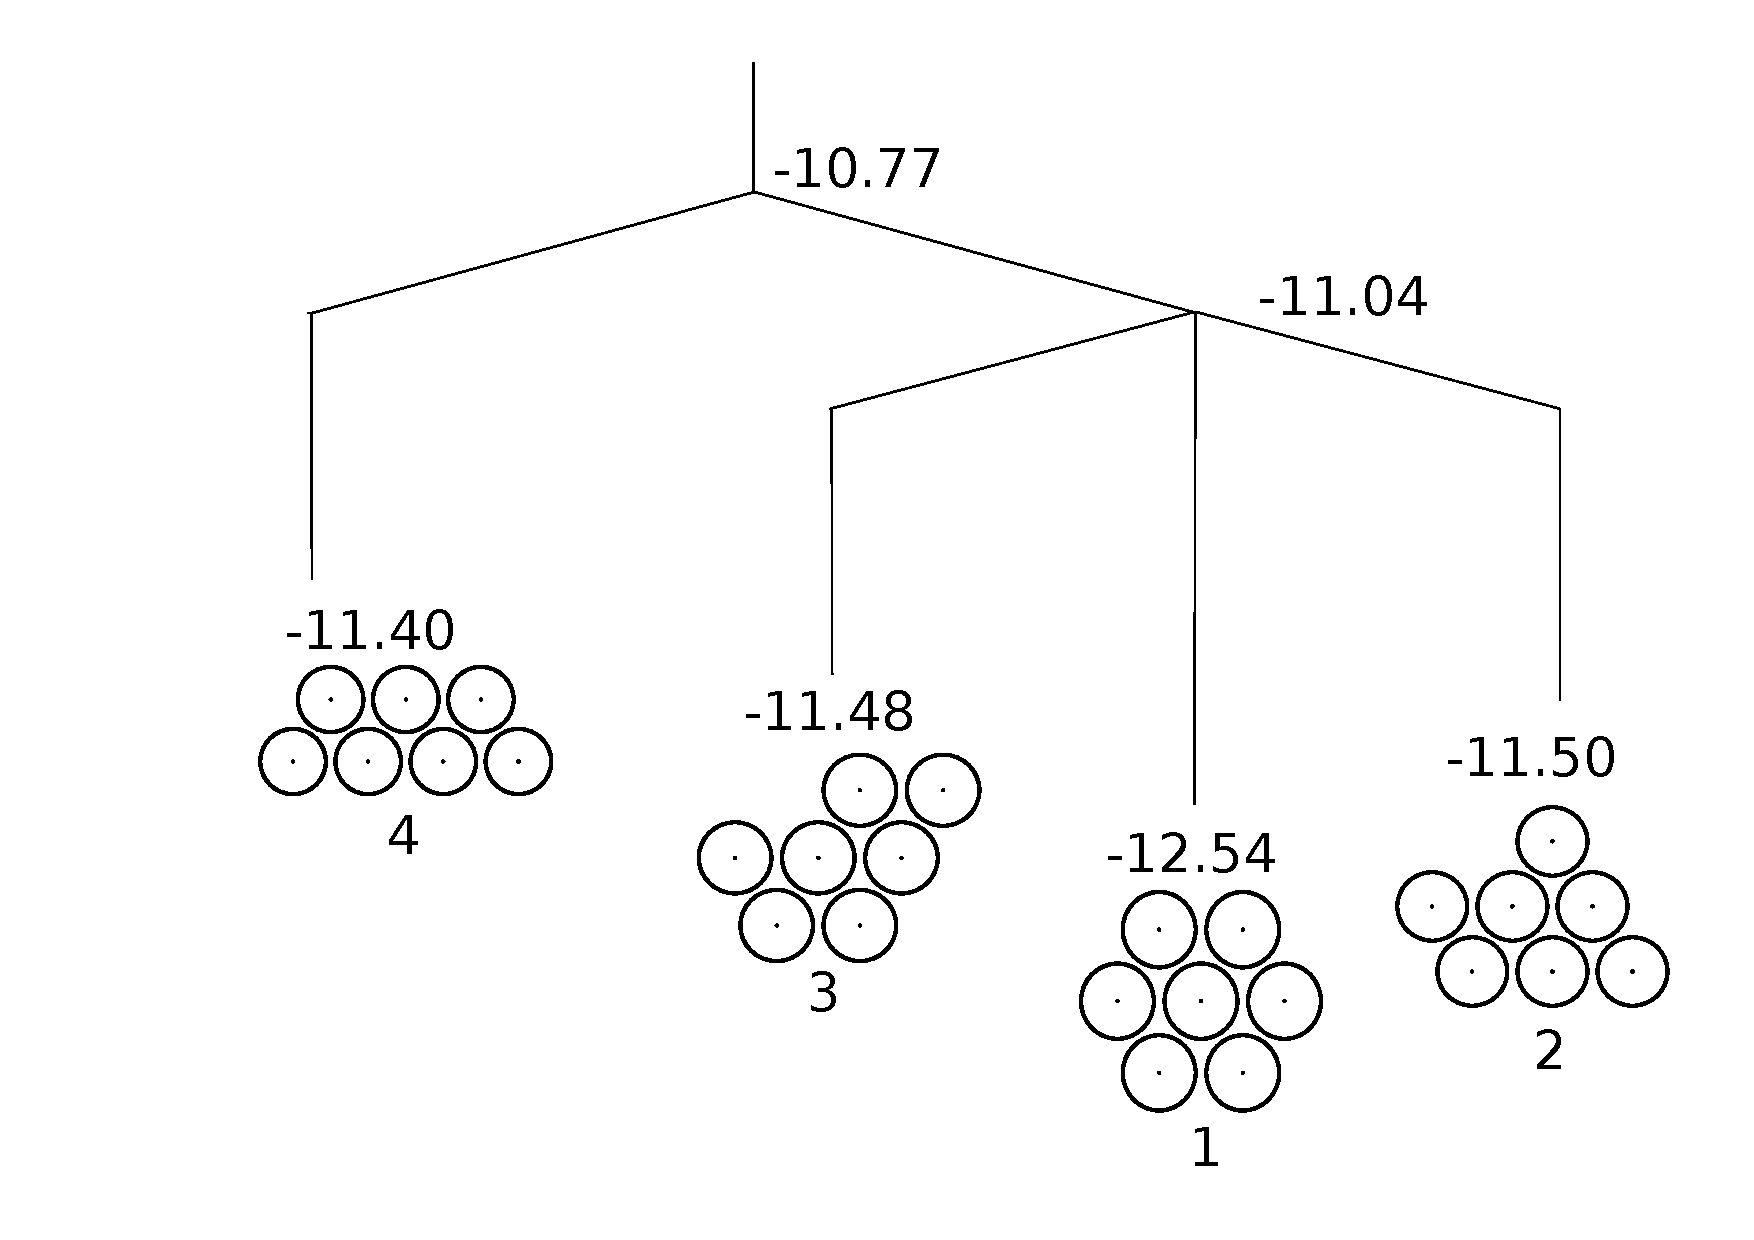
\includegraphics[height=7cm]{Images/disconnect.pdf}
\caption[Disconnectivity graph of ${\rm LJ_7^{2D}}$]{Minima and transition states of the ${\rm LJ_7^{2D}}$ system.\cite{Wales2002, Wales2003} Energies are in reduced units ($\epsilon$). The index of each minimum in order of increasing energy from the global minimum is given below each structure.}
\label{fig:discon-graph}
\end{figure}

\subsection{Implementation}
\label{sec:ljimple}

Calculations using boxes defined by minima only gives a good value for the rate constant $k_{3 \rightarrow 2}$ (transition from minimum 3 to minimum 2, see figure \ref{fig:discon-graph}) but the other rate constants, such as $k_{1 \rightarrow 2}$, are so low that the simulation would be too computationally expensive.
Therefore, the box centres were instead defined as points on pathways in configuration space between the minima.
The pathways were obtained using the doubly-nudged elastic band (DNEB) method \cite{Trygubenko2004} in the \mbox{OPTIM\cite{OPTIM}} program.
A modified L-BFGS minimiser\cite{Nocedal1980} was used for optimisation of the positions of the images along the path.
The points from each path were selected so that the energy difference between each two following points was always less than 0.6.
Redundant points shared by more pathways or very close in energy and RMSD were removed.
In the end, three different configuration space partitionings were used using 4, 13 and 22 boxes.
The structures of the box centres for the partitioning using 22 boxes with their energies is shown in figure \ref{fig:boxes}.

\begin{figure}[h]
\centering
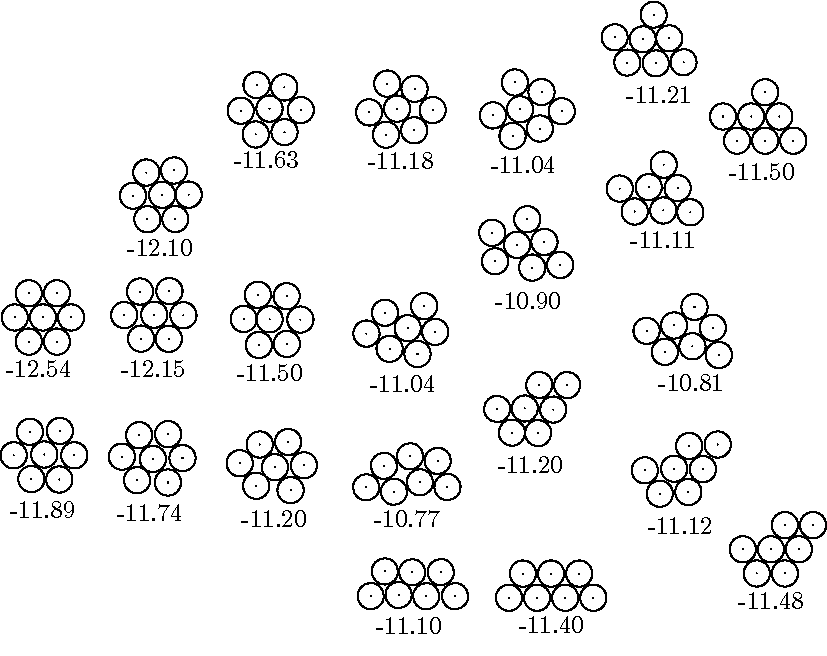
\includegraphics[width=12cm]{Images/boxes.pdf}
\caption[Partitioning of configuration space of ${\rm LJ_7^{2D}}$ into boxes.]{Structures representing generating points for boxes in the Voronoi construction. Energies are given below each structure in $\epsilon$. Some structures are very close to the neighbouring box centres (RMSD$< 0.1$) due to the steep potential and the requirement that energy differences of consecutive generating structures on any path cannot be higher than 0.5 $\epsilon$.}
\label{fig:boxes}
\end{figure}

BXD simulations with boxes defined by Voronoi construction are highly dependent on a fast and reliable calculation of the ``distance".
Out of the possible distance measures, RMSD is the most widely used.
Finding the optimum structural alignment for RMSD calculation with respect to rotational and permutation isomers is a difficult computational problem.
There are efficient algorithms for finding the optimum mutual orientation\cite{Kearsley1989} for a given permutation and for finding the optimum permutation \cite{Kuhn1955, Jonker1987} for a given mutual rotation.
However, the only known deterministic algorithm that ensures convergence to the global minimum of the RMSD with respect to both types of alignment is search over all permutations.
\mbox{GMIN\cite{GMIN}} calculates the RMSD's quickly by applying a modified Hungarian algorithm\cite{Jonker1987} first, followed by optimisation of the mutual rotation.

An alternative alignment method was used in this work.
The centres of mass of two planar structures A and B are first positioned to the same point.
Structure B is then rotated by an angle $\theta$ and the optimum permutation is found using the modified Hungarian algorithm.\cite{Jonker1987}
For the resulting optimum permutation, the angle is optimised with the orthogonal transformation using quaternions.\cite{Kearsley1989}
The application of the Hungarian algorithm and the angle optimisation is performed for $n$ uniformly distributed angles $\theta$ (from 0 to $2 \pi$).
The method neither ensures convergence to the global minimum nor is computationally cheap.
However, the premise that a systematic search through angles will find the global minimum is supported by a known solution to a similar problem.\cite{Helmich2012}
The method was tested on a set of 489 structures representing paths between minima calculated using DNEB.
The results for $n=20$ were identical to the results obtained by the search over all permutations.

The BXD was implemented within the GMIN program\cite{GMIN} as a new procedure BXD2D.
Nose-Hoover \cite{Nose1984, Kleinerman2008} and Berendsen \cite{Berendsen1984} thermostats were used.
The velocity inversion after hitting the wall was performed as in Glowacki {\it et al}.\cite{Glowacki2009}
The rate constants for the transition between particular boxes were calculated using the NGT procedure\cite{Wales2009} implemented in PELE.\cite{pele}

\subsection{Preliminary Results}

The simulation protocol is currently not optimised to yield results comparable to TPS calculations.\cite{Dellago1998b}
Classical simulations in the canonical ensemble of ${\rm LJ_7^{2D}}$ system were performed at $T=0.05$ for evolution times of $10^4$ $\tau_0$.
As mentioned above, the results for four boxes give values comparable to TPS for $k_{3 \rightarrow 2}$, which is large enough to be sampled.
Therefore, the system must be subdivided into more boxes.
The rate constants calculated from simulations with 13 or 22 boxes are significantly higher than the TPS rate constants.


\begin{figure}[h]
\centering
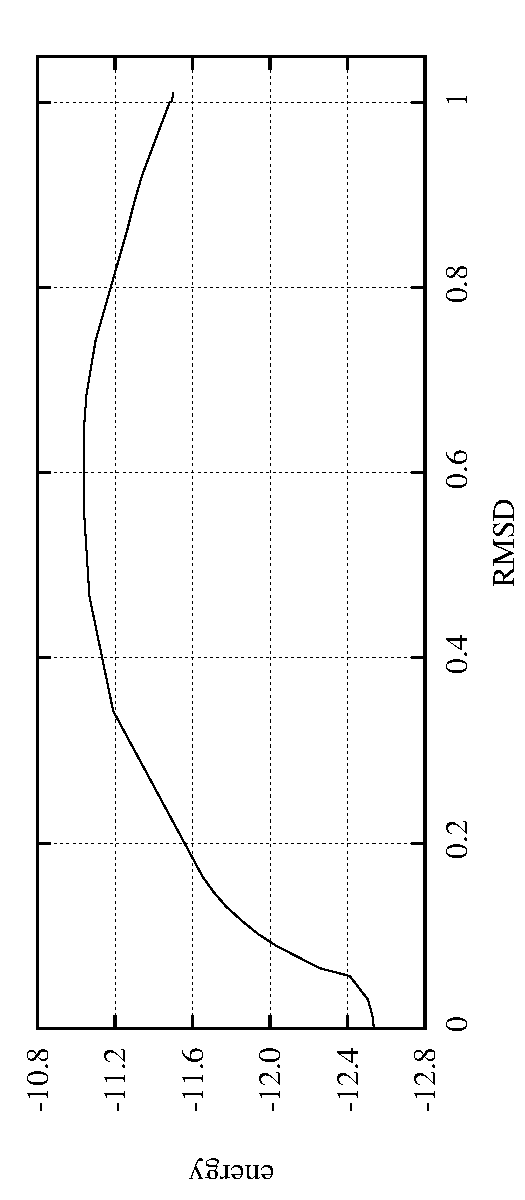
\includegraphics[height=14cm, angle=270]{Images/profileLJ.pdf}
\caption[Energy profile of the configuration transition of ${\rm LJ_7^{2D}}$.]{The energy profile of the transition from minimum 1 (the global minimum) to minimum 2. The RMSD between each point of the path and minimum 1 is calculated using the new method described in section \ref{sec:ljimple}.}
\label{fig:profile}
\end{figure}

The check for Markovianity proposed in section \ref{sec:error} showed that the input and output trajectories are strongly correlated in case of the partitioning into 22 boxes.
First, the system is too simple to sufficiently decorrelate the input and output trajectories.
It is obvious from figure \ref{fig:boxes} that the RMSD's between some box centres are very small.
The energy increases very quickly with RMSD ($5 ~ \epsilon / \sigma$, see figure \ref{fig:profile}) along the transition path from minimum 1 to any other minimum.
Second, as mentioned in section \ref{sec:error}, the inversion procedure by Glowacki {\it et al.}\cite{Glowacki2009} does not preserve the equilibrium distribution and significantly increases the number of the inversion events.
Randomisation of velocities is more difficult to implement for this system.
These problems will hopefully to be resolved in the near future.

